% Options for packages loaded elsewhere
\PassOptionsToPackage{unicode}{hyperref}
\PassOptionsToPackage{hyphens}{url}
\PassOptionsToPackage{dvipsnames,svgnames,x11names}{xcolor}
%
\documentclass[
  letterpaper,
  DIV=11,
  numbers=noendperiod]{scrartcl}

\usepackage{amsmath,amssymb}
\usepackage{lmodern}
\usepackage{iftex}
\ifPDFTeX
  \usepackage[T1]{fontenc}
  \usepackage[utf8]{inputenc}
  \usepackage{textcomp} % provide euro and other symbols
\else % if luatex or xetex
  \usepackage{unicode-math}
  \defaultfontfeatures{Scale=MatchLowercase}
  \defaultfontfeatures[\rmfamily]{Ligatures=TeX,Scale=1}
\fi
% Use upquote if available, for straight quotes in verbatim environments
\IfFileExists{upquote.sty}{\usepackage{upquote}}{}
\IfFileExists{microtype.sty}{% use microtype if available
  \usepackage[]{microtype}
  \UseMicrotypeSet[protrusion]{basicmath} % disable protrusion for tt fonts
}{}
\makeatletter
\@ifundefined{KOMAClassName}{% if non-KOMA class
  \IfFileExists{parskip.sty}{%
    \usepackage{parskip}
  }{% else
    \setlength{\parindent}{0pt}
    \setlength{\parskip}{6pt plus 2pt minus 1pt}}
}{% if KOMA class
  \KOMAoptions{parskip=half}}
\makeatother
\usepackage{xcolor}
\usepackage[left=1in,right=1in,top=1in]{geometry}
\setlength{\emergencystretch}{3em} % prevent overfull lines
\setcounter{secnumdepth}{-\maxdimen} % remove section numbering
% Make \paragraph and \subparagraph free-standing
\ifx\paragraph\undefined\else
  \let\oldparagraph\paragraph
  \renewcommand{\paragraph}[1]{\oldparagraph{#1}\mbox{}}
\fi
\ifx\subparagraph\undefined\else
  \let\oldsubparagraph\subparagraph
  \renewcommand{\subparagraph}[1]{\oldsubparagraph{#1}\mbox{}}
\fi


\providecommand{\tightlist}{%
  \setlength{\itemsep}{0pt}\setlength{\parskip}{0pt}}\usepackage{longtable,booktabs,array}
\usepackage{calc} % for calculating minipage widths
% Correct order of tables after \paragraph or \subparagraph
\usepackage{etoolbox}
\makeatletter
\patchcmd\longtable{\par}{\if@noskipsec\mbox{}\fi\par}{}{}
\makeatother
% Allow footnotes in longtable head/foot
\IfFileExists{footnotehyper.sty}{\usepackage{footnotehyper}}{\usepackage{footnote}}
\makesavenoteenv{longtable}
\usepackage{graphicx}
\makeatletter
\def\maxwidth{\ifdim\Gin@nat@width>\linewidth\linewidth\else\Gin@nat@width\fi}
\def\maxheight{\ifdim\Gin@nat@height>\textheight\textheight\else\Gin@nat@height\fi}
\makeatother
% Scale images if necessary, so that they will not overflow the page
% margins by default, and it is still possible to overwrite the defaults
% using explicit options in \includegraphics[width, height, ...]{}
\setkeys{Gin}{width=\maxwidth,height=\maxheight,keepaspectratio}
% Set default figure placement to htbp
\makeatletter
\def\fps@figure{htbp}
\makeatother

\setkomafont{author}{\small}
\setkomafont{date}{\small}
\KOMAoption{captions}{tableheading}
\makeatletter
\makeatother
\makeatletter
\makeatother
\makeatletter
\@ifpackageloaded{caption}{}{\usepackage{caption}}
\AtBeginDocument{%
\ifdefined\contentsname
  \renewcommand*\contentsname{Table of contents}
\else
  \newcommand\contentsname{Table of contents}
\fi
\ifdefined\listfigurename
  \renewcommand*\listfigurename{List of Figures}
\else
  \newcommand\listfigurename{List of Figures}
\fi
\ifdefined\listtablename
  \renewcommand*\listtablename{List of Tables}
\else
  \newcommand\listtablename{List of Tables}
\fi
\ifdefined\figurename
  \renewcommand*\figurename{Figure}
\else
  \newcommand\figurename{Figure}
\fi
\ifdefined\tablename
  \renewcommand*\tablename{Table}
\else
  \newcommand\tablename{Table}
\fi
}
\@ifpackageloaded{float}{}{\usepackage{float}}
\floatstyle{ruled}
\@ifundefined{c@chapter}{\newfloat{codelisting}{h}{lop}}{\newfloat{codelisting}{h}{lop}[chapter]}
\floatname{codelisting}{Listing}
\newcommand*\listoflistings{\listof{codelisting}{List of Listings}}
\makeatother
\makeatletter
\@ifpackageloaded{caption}{}{\usepackage{caption}}
\@ifpackageloaded{subcaption}{}{\usepackage{subcaption}}
\makeatother
\makeatletter
\@ifpackageloaded{tcolorbox}{}{\usepackage[many]{tcolorbox}}
\makeatother
\makeatletter
\@ifundefined{shadecolor}{\definecolor{shadecolor}{rgb}{.97, .97, .97}}
\makeatother
\makeatletter
\makeatother
\ifLuaTeX
  \usepackage{selnolig}  % disable illegal ligatures
\fi
\IfFileExists{bookmark.sty}{\usepackage{bookmark}}{\usepackage{hyperref}}
\IfFileExists{xurl.sty}{\usepackage{xurl}}{} % add URL line breaks if available
\urlstyle{same} % disable monospaced font for URLs
\hypersetup{
  pdftitle={Hypothesis testing with Randomization},
  pdfauthor={Practice problems},
  colorlinks=true,
  linkcolor={blue},
  filecolor={Maroon},
  citecolor={Blue},
  urlcolor={Blue},
  pdfcreator={LaTeX via pandoc}}

\title{Hypothesis testing with Randomization}
\author{Practice problems}
\date{10/16/24}

\begin{document}
\maketitle
\ifdefined\Shaded\renewenvironment{Shaded}{\begin{tcolorbox}[breakable, frame hidden, borderline west={3pt}{0pt}{shadecolor}, enhanced, interior hidden, sharp corners, boxrule=0pt]}{\end{tcolorbox}}\fi

\begin{enumerate}
\def\labelenumi{\arabic{enumi}.}
\item
  The Stanford University Heart Transplant Study was conducted to
  determine whether an experimental heart transplant program increased
  lifespan. Each patient entering the program was designated an official
  heart transplant candidate, meaning that they were gravely ill and
  would most likely benefit from a new heart. Some patients got a
  transplant and some did not. The variable \texttt{transplant}
  indicates which group the patients were in: treatment (received
  transplant) or control (no transplant). The variable \texttt{survived}
  indicates whether the patient was alive at the end of the study or
  died. Of the 34 patients in the control group, 30 died. Of the 69
  people in the treatment group, 45 died.

  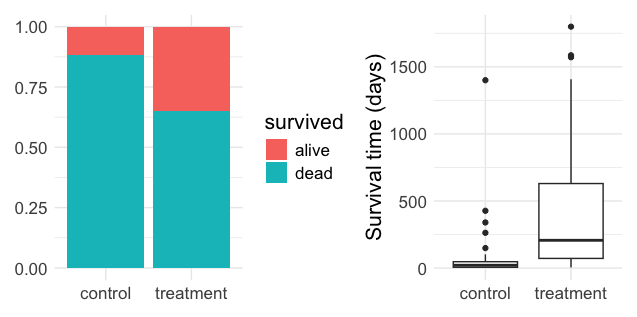
\includegraphics[width=4.14583in,height=\textheight]{images/14-heart-transplant-eda.png}

  \begin{enumerate}
  \def\labelenumii{\alph{enumii}.}
  \item
    What do the two plots above suggest about 1) if survival is
    independent of receiving a transplant and 2) the efficacy of heart
    transplants? Explain your reasoning.
  \item
    What proportion of patients in the treatment group and the control
    group died?
  \item
    Write out a null and alternative hypothesis for investigating
    whether there is statistically significant evidence that the
    treatment is effective.
  \item
    The paragraph below describes the set up for a randomization test if
    we did not have access to software. Fill in the blanks with a number
    or phrase using your answers to (b) and (c) for guidance:

    We write the word \_\_\_\_\_\_ on \_\_\_\_\_\_\_ cards representing
    patients who were alive at the end of the study, and \_\_\_\_\_\_ on
    \_\_\_\_\_\_ cards representing the patients who were not. Then we
    shuffle these cards and split them into two groups: one group of
    size \_\_\_\_\_\_ representing treatment, and one group of size
    \_\_\_\_\_\_ representing \_\_\_\_\_\_\_\_\_. We calculate the
    difference between the proportion of \_\_\_\_\_\_\_\_ cards in the
    treatment and control groups (treatment - control) and record this
    value. We repeat this 1000 times to build a distribution centered at
    \_\_\_\_\_\_\_. This is called the \_\_\_\_\_\_\_\_ distribution.
    Lastly, we calculate the proportion of simulations where the
    simulated difference in proportions are \_\_\_\_\_\_\_\_\_. If this
    proportion is low, we conclude that that it is \_\_\_\_\_\_\_\_\_\_
    to have observed our data by chance assuming \_\_\_\_\_\_\_\_\_\_\_.
  \item
    What do the simulation results shown below suggest about the
    effectiveness of heart transplants?

    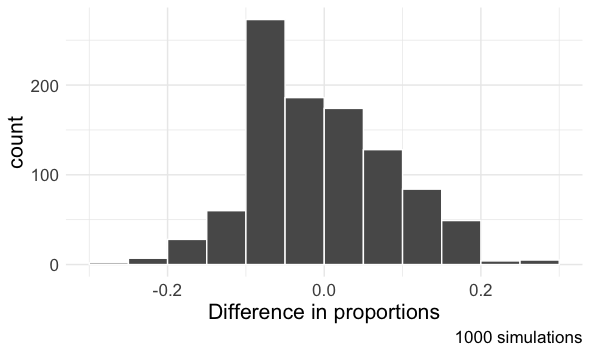
\includegraphics[width=4.51042in,height=\textheight]{images/14-heart-transplant-null.png}
  \item
    Suggest a more informative x-axis label for the plot above.
  \end{enumerate}
\item
  Understanding cultural differences in tobacco use across different
  demographic groups can lead to improved health care education and
  treatment. A recent study dis-aggregated tobacco use across Asian
  American ethnic groups, including Asian-Indian (n = 4373), Chinese (n
  = 4736), and Filipino (n = 4912), in comparison to non-Hispanic Whites
  (n = 275025). The number of current smokers in each group at the time
  of study was reported as:

  \begin{itemize}
  \item
    Asian-Indian: 223
  \item
    Chinese: 279
  \item
    Filipino: 609
  \item
    non-Hispanic Whites: 50880
  \end{itemize}

  To determine whether the proportion of Asian-Indian Americans who are
  current smokers is different from the proportion of Chinese Americans
  who are smokers, a randomization simulation was performed.

  \begin{enumerate}
  \def\labelenumii{\alph{enumii}.}
  \item
    Using both symbols and words, provide the parameter and statistic of
    interest for this study. Do you know the numerical value of either
    the parameter or statistic of interest? If so, provide it.
  \item
    The histogram below provides the simulated null distribution
    obtained from 1000 repetitions. Estimate the standard error.

    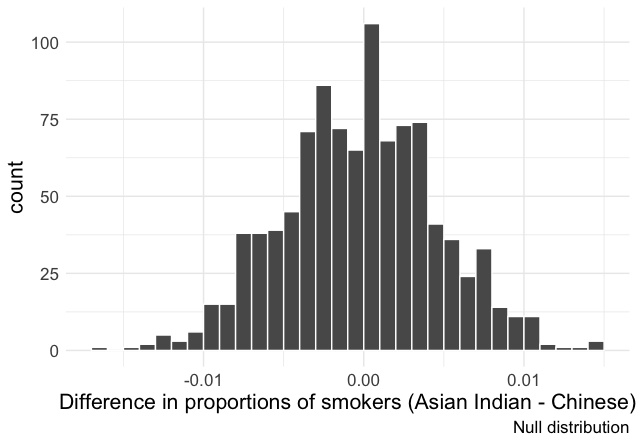
\includegraphics[width=3.65625in,height=\textheight]{images/14-asian-tobacco-null.png}
  \item
    Consider the hypothesis test to determine if there is a difference
    in proportion of Asian-Indian Americans as compared to Chinese
    Americans who are current smokers. Write out the null and
    alternative hypotheses, and estimate a p-value using the
    randomization histogram from (b). If the significance level is
    \(\alpha = 0.05\), what is your decision and conclusion in the
    context of the problem?
  \item
    Now consider the following bootstrap distribution of the difference
    in sample proportions of current smokers (Filipino Americans minus
    Chinese Americans) in 1000 repetitions. Find a 95\% bootstrap
    confidence interval for the true difference in the proportion of
    current smokers in the population. Interpret the interval in the
    context of the problem, assuming our sample is representative.

    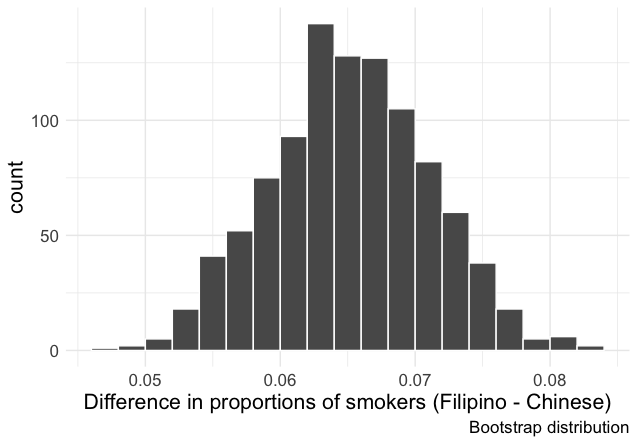
\includegraphics[width=3.63542in,height=\textheight]{images/14-asian-tobacco-boot.png}
  \end{enumerate}
\end{enumerate}



\end{document}
